\section*{2.2 Método punto fijo o sustitución sucesiva}

Un punto fijo para una función es un número en el que el valor de la función no cambia cuando se aplica la función.
\\

\begin{tcolorbox}[colback=gray!5!]
\subsubsection*{Definición}
El número \textit{p} es un \textbf{punto fijo} de una función dada $g$ si $g(p)=p$.
\end{tcolorbox}

En esta sección consideraremos el problema de encontrar soluciones mediante punto fijo y su conexión con los problemas de encontrar raíces. Ambos son de similares en el siguiente sentido:

\begin{itemize}
    \item Dado el problema de encontrar la raíz de $f(p)=0$, podemos definir las funciones $g$  con un punto fijo en $p$ de varias formas, por ejemplo: 
    \begin{center}
        $g(x)=x-f(x)$ o como $g(x)=x +3f(x)$.
    \end{center}
    \item Por el contrario si la función $g$ tiene un punto fijo en $p$, entonces la función definida por 
    \begin{equation*}
        f(x)=x-g(x)
    \end{equation*}
    tiene un cero en $p$.
\end{itemize}

Aunque los problemas que deseamos están en la forma de búsqueda de raíces, la forma de punto fijo es más fácil de analizar, y ciertas elecciones de punto fijo conducen a una técnicas de búsqueda de raíz poderosas.

\subsubsection*{Ejemplo}
Determine cualquier punto fijo de la función $g(x)=x^2-2$.

\textbf{Solución}. Un punto fijo de g tiene la propiedad de 
\begin{center}
    $p=g(p)=p^2-2$ lo cual implica que $0=p^2-p-2=(p+1)(p-2)$.
\end{center}

Un punto fijo de $g$ ocurre precisamente cuando la gráfica de $y=g(x)$ corta en $y=x$, entonces $g$ tiene dos puntos fijos, uno en $p=-1$ y otro en $p=2$ como se muestra. \ref{tab:fig}

\begin{figure*}[h!]
\centering
  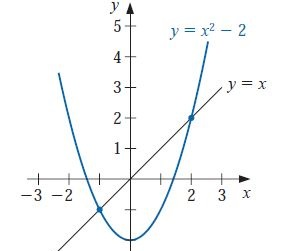
\includegraphics[width=0.6\textwidth]{Puntofijo.JPG}
\caption{Punto fijo}
\label{tab:fig}
\end{figure*} 


Por otra parte, cuando no podamos determinar el punto fijo de alguna función porque no podamos resolver para $p$ dicha ecuación se considerarán aproximaciones con precisión determinada. A continuación se muestra como hacerlo.

Para aproximar el punto dijo de una función $g$ elegimos una aproximación inicial $p_0$ y generamos la secuencia $\left\lbrace p_n\right\rbrace ^\infty_{n=0}$ siendo $p_n=g(p_{n-1})$, para cada $n>1$. Si la secuencia converge a $p$ y $g$ es continua, entonces

\begin{equation*}
    p = \lim_{n \to \infty}(p_n)=\lim_{n \to \infty}g(p_{n-1})=g\left(\lim_{n \to \infty}(p_{n-1})\right)=g(p),
\end{equation*}

Y se obtiene una solución a $x=g(x)$. Esta técnica es llamada \textbf{punto fijo}. El procedimiento se ilustra en \ref{tab:fig2}:

\begin{figure*}[h!]
\centering
  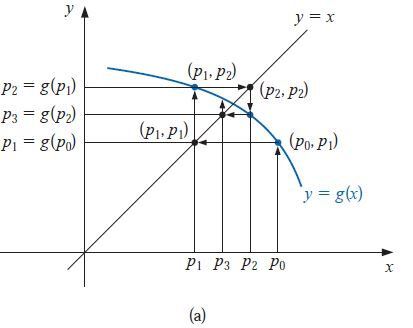
\includegraphics[width=0.6\textwidth]{Puntofijo2.JPG}
\caption{Punto fijo 2}
\label{tab:fig2}
\end{figure*} 

\begin{tcolorbox}[colback=blue!15!]
\subsubsection*{Punto fijo}
Para encontrar la solución a $p=g(p)$ dada la aproximación inicial $p_0$:
\\ \\
ENTRADA aproximación inicial $p_0$; tolerancia \textit{TOL}; número máximo de iteraciones $N_0$.

SALIDA La solución aproximada \textit{p} o mensaje de falla.

PASO 1 Asigna i=1;

PASO 2 Mientras $i\leq N_0$ ejecuta los pasos 3-6.

\ \ \ \  PASO 3 Asigna $p=g(p_0)$; (calcula $p_i$)

\ \ \ \  PASO 4 Si $|p-p_0|<TOL$ entonces

\ \ \ \ \ \ \ \ \ \ \ \ \ \ \ \ \ \ SALIDA (p); (proceso completado exitosamente)

\ \ \ \ \ \ \ \ \ \ \ \ \ \ \ \ \ \ ALTO.

\ \ \ \   PASO 5 Asigna $i=i+1$
    
\ \ \ \   PASO 6 Asigna $p_0=p$; (Actualiza $p_0$.)

PASO 7 SALIDA ('El método fallo después de $N_0$ iteraciones $N_0=$',$N_0$);

\ \ \ \ \ \ \ \ \ \ \ \ \ (El proceso fue exitoso.)

\ \ \ \ \ \ \ \ \ \ \ \ \ ALTO.


\end{tcolorbox}

A continuación se ilustran algunas características de la iteración funcional.

\subsubsection*{Ejemplo}
La ecuación $x^3+4x^2-10=0$ tiene una única raíz en $[1,2]$. Hay muchas formas de cambiar la ecuación para la forma de punto fijo $x=g(x)$ utilizando simple manipulación algebraica. Por ejemplo, para obtener la función $g$ descrita en el inciso (c) se manipula la ecuación $x^3+4x^2-10=0$ como a continuación:

\begin{center}
$4x^2=10-x^3$, entonces $x^2=\frac{1}{4}(10-x^3)$ y $x=\pm\frac{1}{2}(10-x^3)^{1/2}$
\end{center}

\begin{tcolorbox}[colback=gray!5!]
\subsubsection*{Nota}
Es importante resaltar que no todas las formas llevan a convergencia aunque todas son soluciones de la ecuación original, por ejemplo:
\end{tcolorbox}

\quad\quad\quad \textbf{(a)} $x=g_1(x)=x-x^3-4x^2+10$
\quad\quad\quad \textbf{(b)} $x=g_2(x)=(\frac{10}{x}-4x)^{1/2}$

\quad\quad\quad \textbf{(c)} $x=g_3(x)=\frac{1}{2}(10-x^3)^{1/2}$
\quad\quad\quad \textbf{(d)} $x=g_4(x)=(\frac{10}{x+4})^{1/2}$

\quad\quad\quad \textbf{(e)} $x=g_5(x)=x-\frac{x^3+4x^2-10}{3x^2+8x}$
\\
\\

Con $p_0=1.5$ se obtiene la tabla \ref{tab:tabla4}:

\begin{table}[h!]
\centering
    \begin{tabular}{||c c c c c c||}
    \hline 
    \hline
        n & (a) & (b) & (c) & (d) & (e) \\
    \hline 
    \hline 
        0 & 1.5 & 1.5 & 1.5 & 1.5 & 1.5 \\
        1 & −0.875 & 0.8165 & 1.286953768 & 1.348399725 &  1.373333333 \\
        2 & 6.732 & 2.9969 & 1.402540804 & 1.367376372 & 1.365262015 \\
        3 & −469.7 & $−8.65^{1/2}$ & 1.345458374 & 1.364957015 &  1.365230014 \\
        4 & $1.03\times10^{8}$ &  & 1.375170253 & 1.365264748 &  1.365230013 \\
        5 &  &  & 1.360094193 & 1.365225594 & \\
        6 &  &  & 1.367846968 & 1.365230576 & \\
        7 &  &  & 1.363887004 & 1.365229942 & \\
        8 &  &  & 1.365916734 & 1.365230022 & \\
        9 &  &  & 1.364878217 & 1.365230012 & \\
        10 &  &  & 1.365410062 & 1.365230014 & \\
        15 &  &  & 1.365223680 & 1.365230013 & \\
        20 &  &  & 1.365230236 &  & \\
        25 &  &  & 1.365230006 &  & \\
        30 &  &  & 1.365230013 &  & \\
        \hline
        \hline 
    \end{tabular}
    \caption{Punto fijo}
    \label{tab:tabla4}
\end{table}


La raíz real es 1.365230013. Comparando el resultados del algoritmo de bisección dado en ese ejemplo, se puede ver que los resultados excelentes se han obtenido para las opciones (c), (d) y (e) (el método de bisección requiere 27 iteraciones para esta precisión). Es interesante notar que la elección (a) fue divergente y que (b) se convirtió en indefinido porque involucra la raíz cuadrada de un número negativo. 